\subsection{Histogram analysis}
\label{sec:histogram_analysis}

\subsection{Distribution of Random Bits Generated with Python Random Seeds}
\label{sec:distribution_python_seed}

The distribution results of each technique are separated by the method used to obtain the seed versus the technique used to distill and obtain the random big number, so we can observe different results for each case.

To view the distribution of values, distribution graphs were used, either standard or uniform, depending on the input data. In our experiments, uniform distributions were shown. 8-bit segments were taken, dividing the entire input data set into byte blocks, obtaining bytes from 0 to 255. This range of possibilities gives us a visual of how the results are distributed.

We begin with the first technique, which was the generation of 6.25 million 32-byte seeds that were used to generate 6.25 million random bytes, or 50 million random bits, using the \textit{CTR\_DRBG} technique. The graph we see below leads us to the conclusion that there is a uniform distribution of the results without pronounced peaks, which are a symptom of an effective system in generating random bits.

\begin{figure}[htbp]
    \centering
    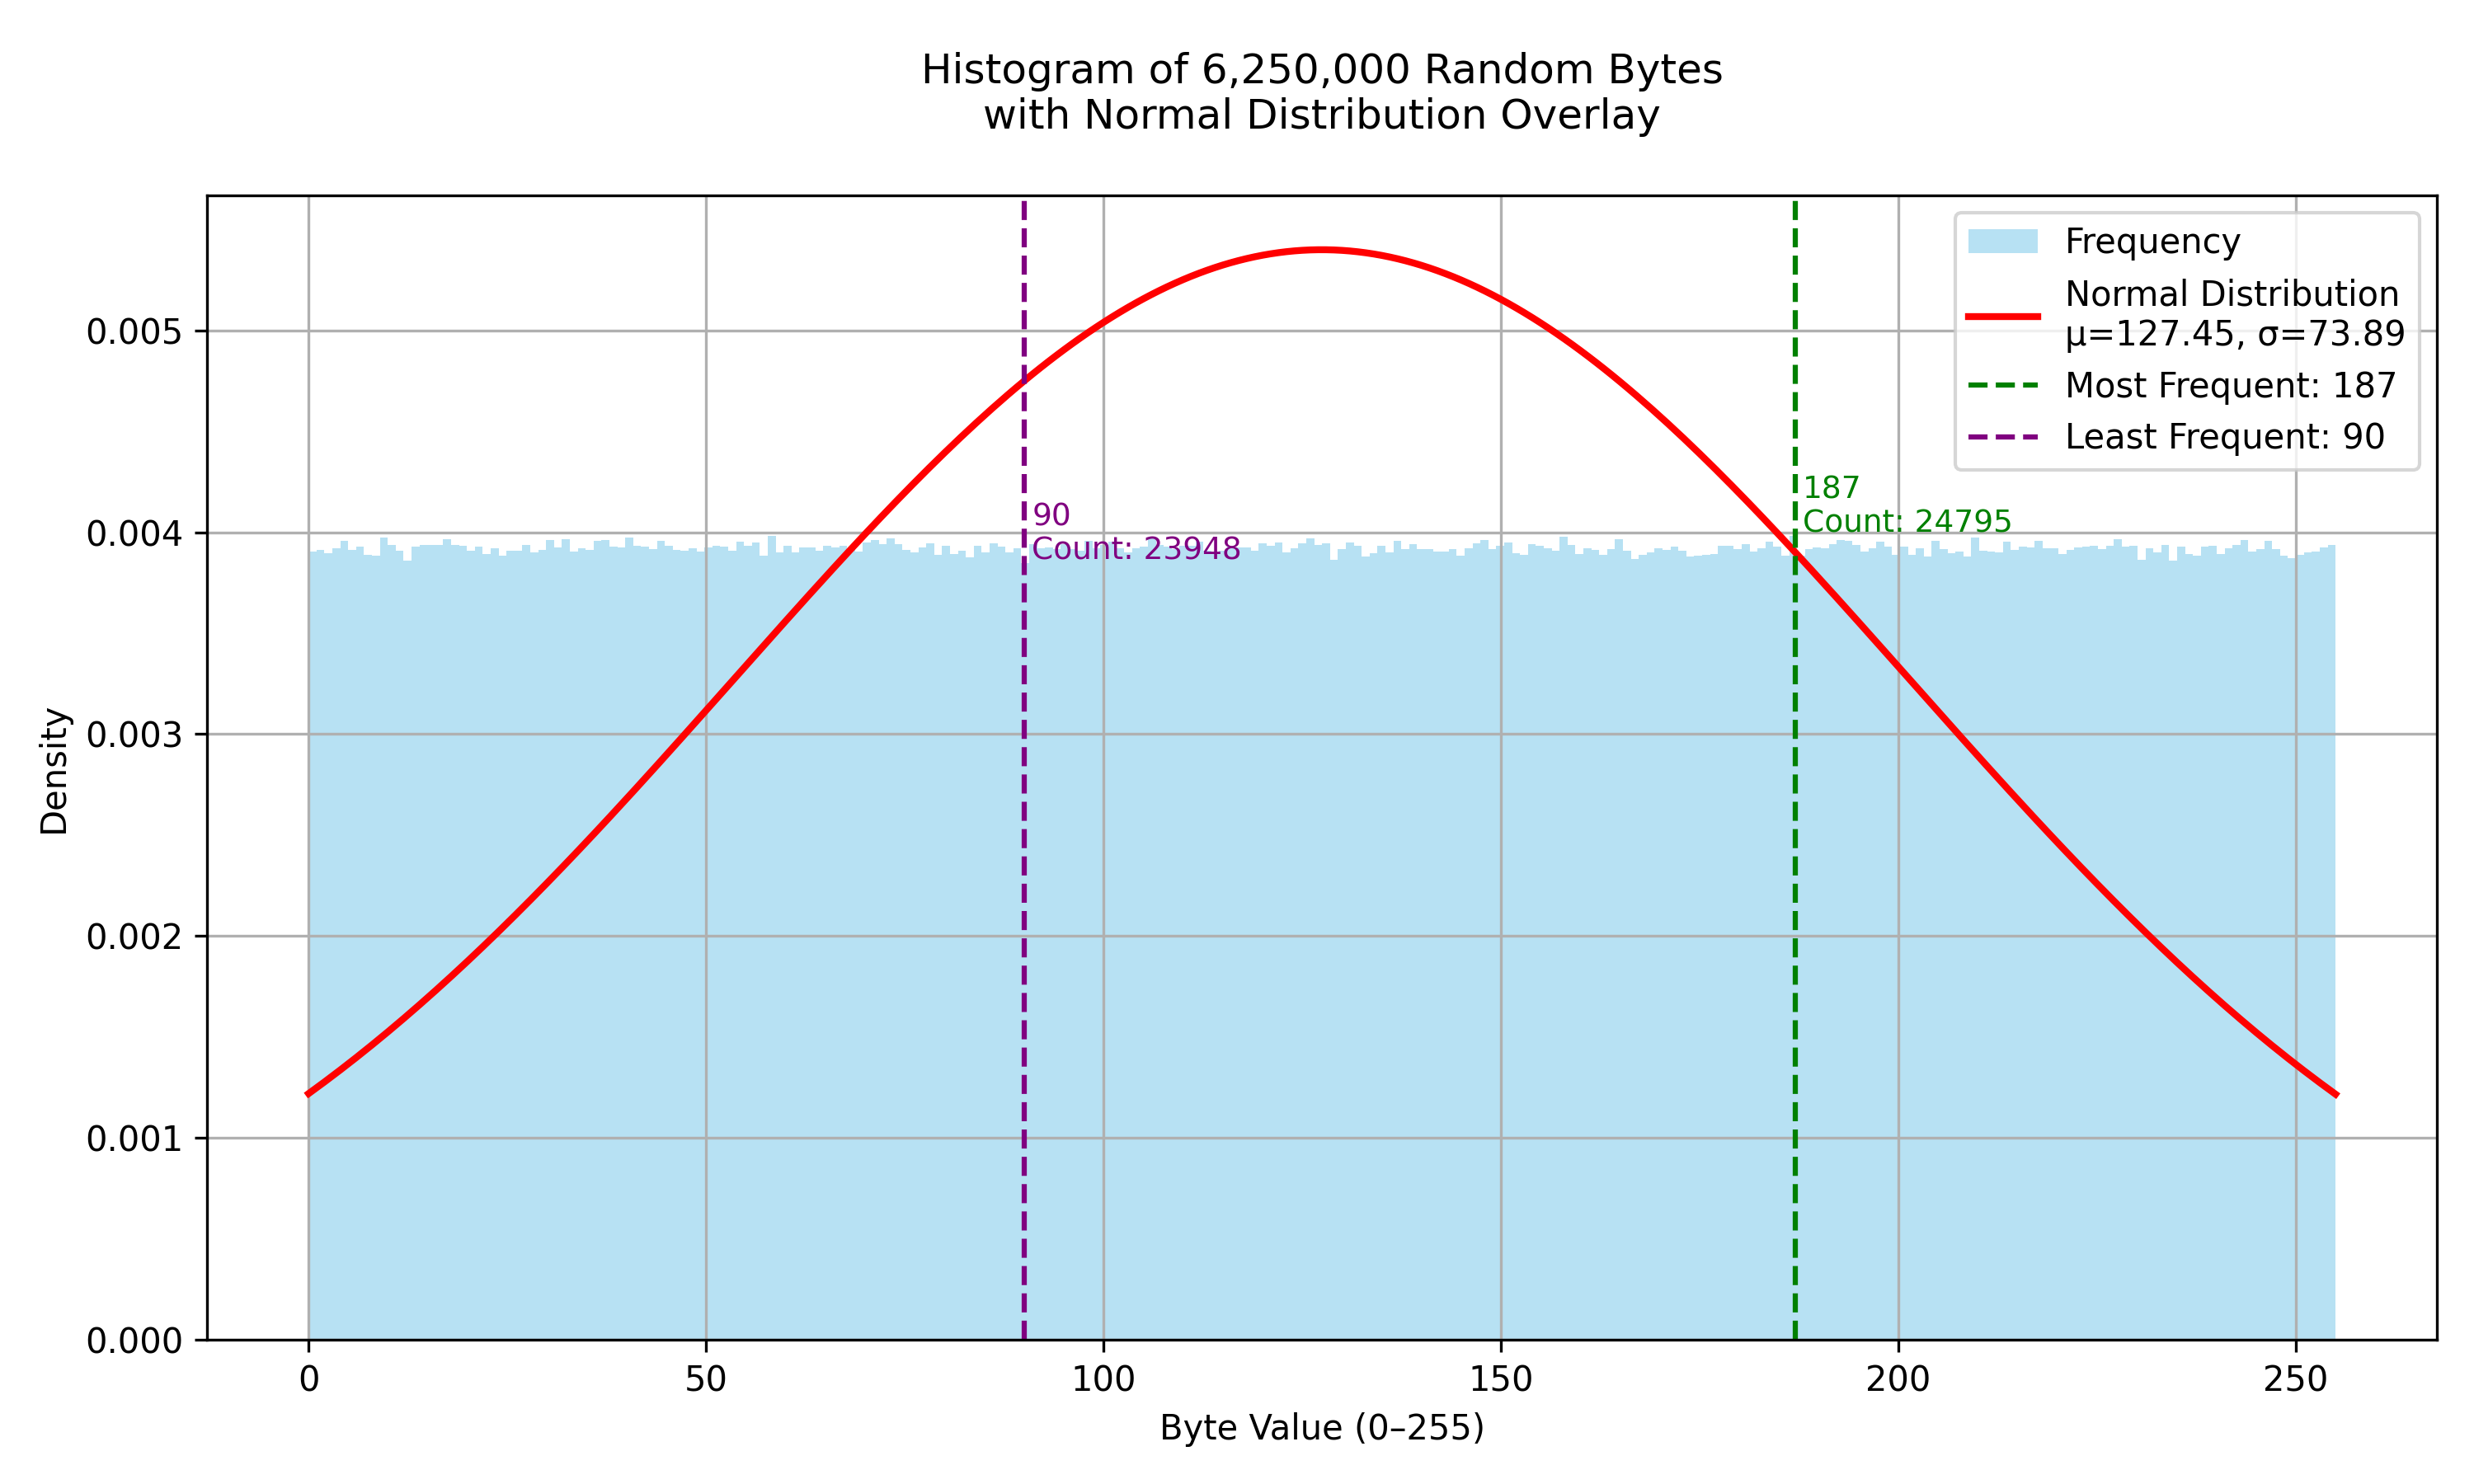
\includegraphics[width=0.9\linewidth]{images/random_bits_CTR_DRBG_seed_python_random.png}
    \caption{\raggedright Random bits \textit{CTR\_DRBG} seed generation with Python random function.}
    \label{fig:ctr_drbg_python_random}
\end{figure}


\subsection{Distribution of Random Bits Generated with Sequential Seeds}
\label{sec:distribution_sequential_seed}

For the following test, sequential seeds were used starting at 1 and reaching 6.5 million in the set of natural numbers. This number was converted to binary and turned into a 32-bit number, then it was used as a seed to generate the distribution with the \textit{CTR\_DRBG} method, showing a uniform distribution without much variation. Unexpectedly, it is seen that the distribution behaves very similar to obtaining reliable seeds with true entropy. Below is the graph.

\begin{figure}[htbp]
    \centering
    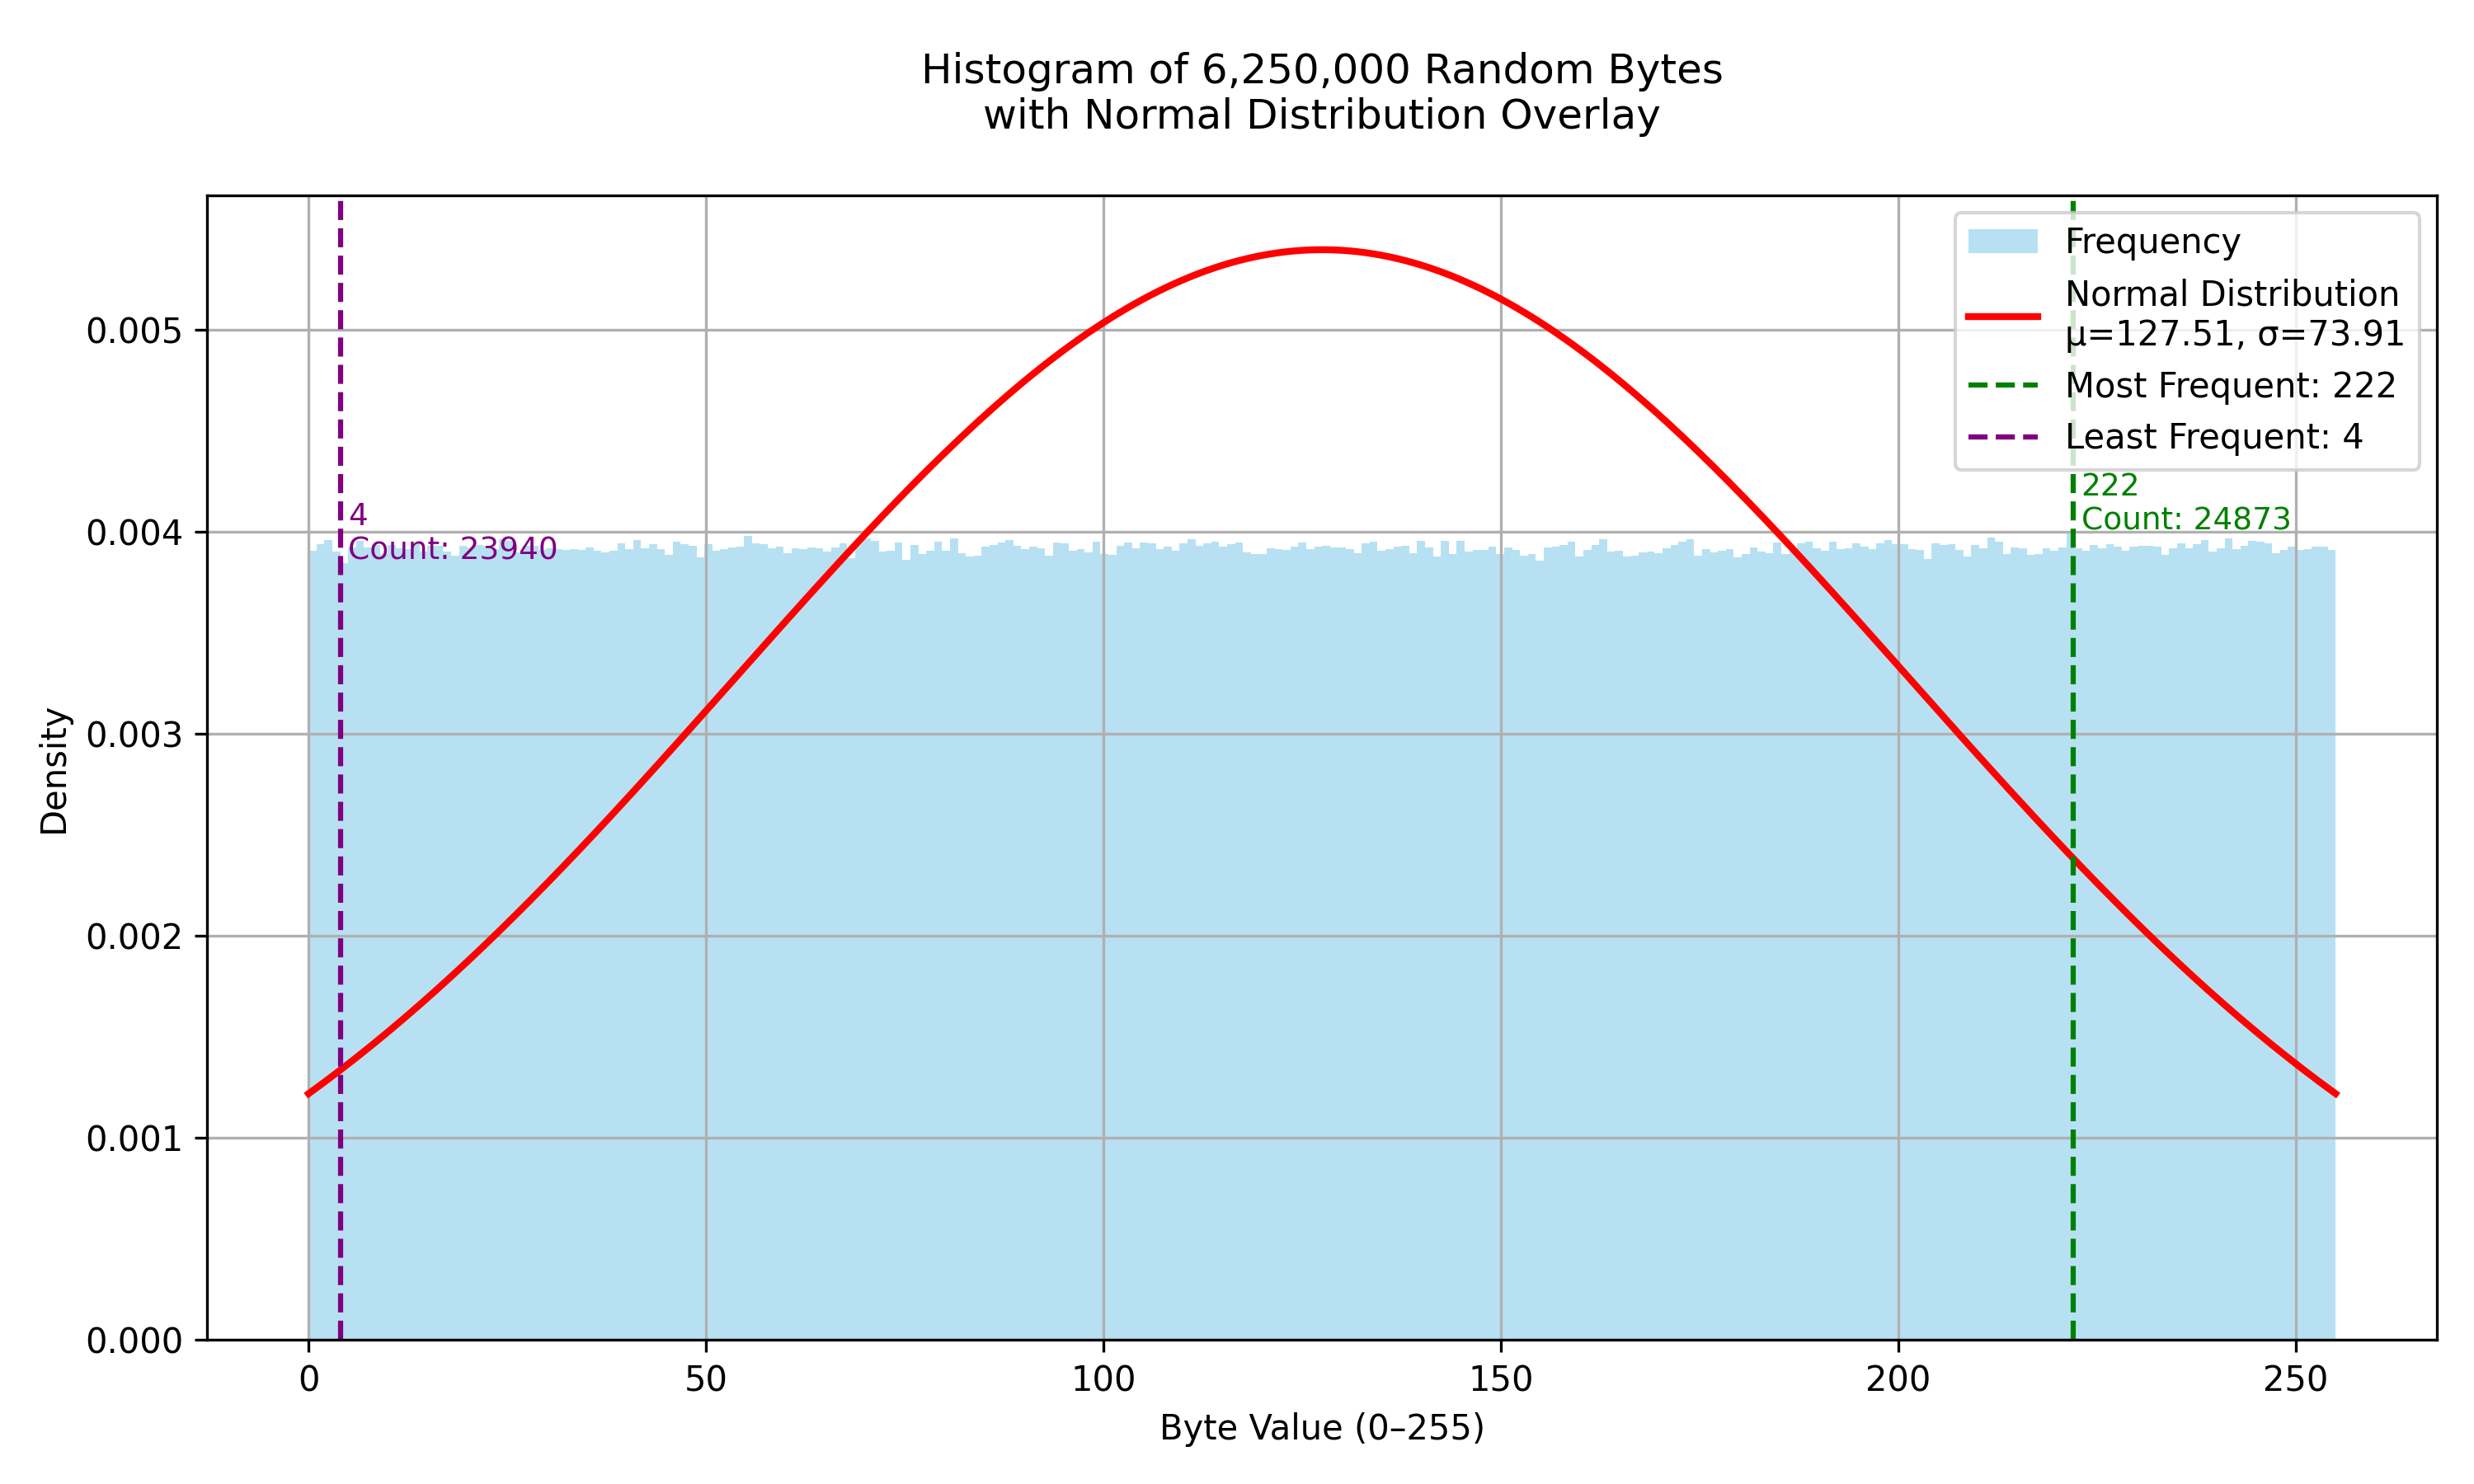
\includegraphics[width=0.9\linewidth]{images/secuentialSeedFrom0_To_100M_CTR_DRBG.png}
    \caption{\raggedright Sequential seed from 1 to 6.5M using \textit{CTR\_DRBG}.}
    \label{fig:ctr_drbg_sequential_seed}
\end{figure}
